\documentclass[main.tex]{subfiles}

\begin{document}

\pagebreak

\section{Aufgabe 4}
Modellieren Sie den klassischen Euklidischen Algorithmus in seiner iterativen Form formal korrekt als Aktivität eines UML-Aktivitätsdiagramms, siehe
\href{https://de.wikipedia.org/wiki/Euklidischer_Algorithmus#Beschreibung_durch_Pseudocode}{Wikipedia: Euklidischer Algorithmus}.
Vergessen Sie dabei nicht, auch die Ein- und Ausgabeparameter und die Datentypen anzugeben.

\subsection{Lösung 4}

\begin{figure}[h!]
    \makebox[\textwidth][c]{
        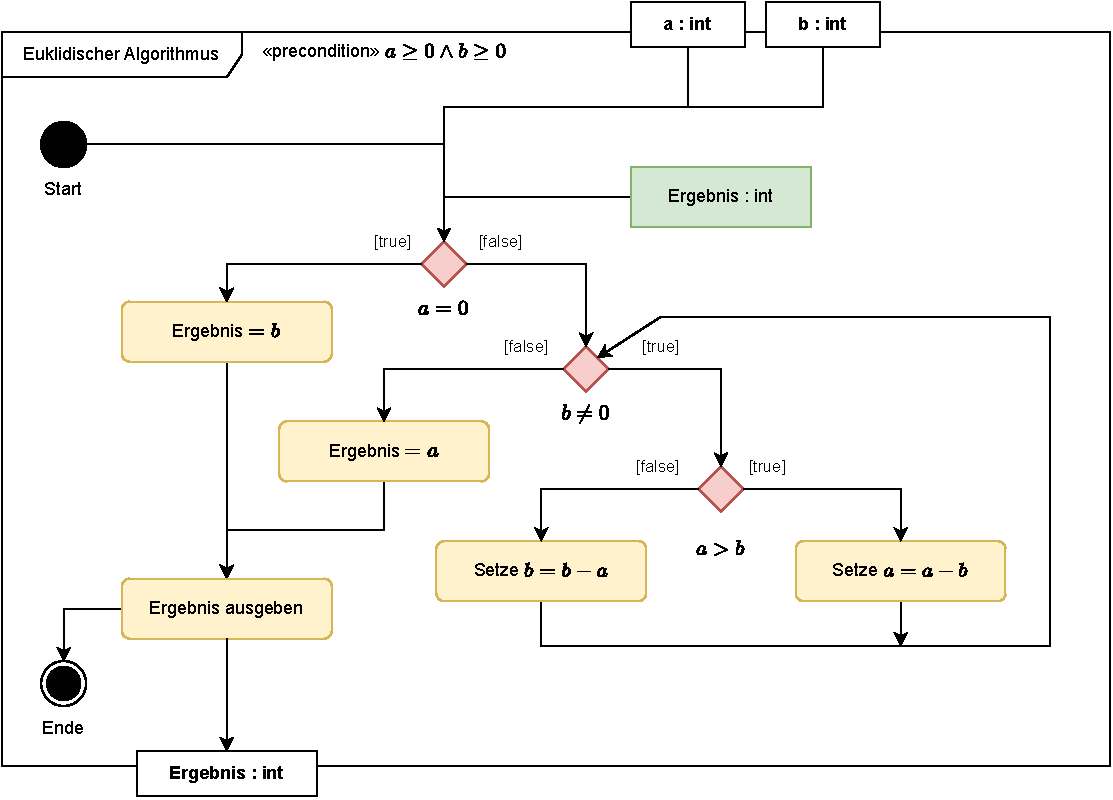
\includegraphics[width=1.2\linewidth]{h03_A4.pdf}
    }
    \caption{Euklidischer Algorithmus}
    \label{fig:lgs4}
\end{figure}

\end{document}
